% !TEX TS-program = pdflatex
% !TEX encoding = UTF-8 Unicode

% This is a simple template for a LaTeX document using the "article" class.
% See "book", "report", "letter" for other types of document.

\documentclass[20pt]{article} % use larger type; default would be 10pt

\usepackage[utf8]{inputenc} % set input encoding (not needed with XeLaTeX)

%%% Examples of Article customizations
% These packages are optional, depending whether you want the features they provide.
% See the LaTeX Companion or other references for full information.

%%% PAGE DIMENSIONS
\usepackage{geometry} % to change the page dimensions
\geometry{a4paper} % or letterpaper (US) or a5paper or....
% \geometry{margin=2in} % for example, change the margins to 2 inches all round
% \geometry{landscape} % set up the page for landscape
%   read geometry.pdf for detailed page layout information

\usepackage{graphicx} % support the \includegraphics command and options

% \usepackage[parfill]{parskip} % Activate to begin paragraphs with an empty line rather than an indent

%%% PACKAGES
\usepackage{booktabs} % for much better looking tables
\usepackage{array} % for better arrays (eg matrices) in maths
\usepackage{paralist} % very flexible & customisable lists (eg. enumerate/itemize, etc.)
\usepackage{verbatim} % adds environment for commenting out blocks of text & for better verbatim
%\usepackage{subfig} % make it possible to include more than one captioned figure/table in a single float
\usepackage{mathtools}
\usepackage{graphicx} % supports images in latex
% These packages are all incorporated in the memoir class to one degree or another...

\usepackage{graphicx}
\usepackage{subcaption}

%%% Other stuff
\DeclarePairedDelimiter\ceil{\lceil}{\rceil}
\DeclarePairedDelimiter\floor{\lfloor}{\rfloor}

%%% HEADERS & FOOTERS
\usepackage{fancyhdr} % This should be set AFTER setting up the page geometry
\pagestyle{fancy} % options: empty , plain , fancy
\renewcommand{\headrulewidth}{0pt} % customise the layout...
\lhead{}\chead{}\rhead{}
\lfoot{}\cfoot{\thepage}\rfoot{}

%%% SECTION TITLE APPEARANCE
\usepackage{sectsty}
\allsectionsfont{\sffamily\mdseries\upshape} % (See the fntguide.pdf for font help)
% (This matches ConTeXt defaults)

%%% ToC (table of contents) APPEARANCE
\usepackage[nottoc,notlof,notlot]{tocbibind} % Put the bibliography in the ToC
\usepackage[titles,subfigure]{tocloft} % Alter the style of the Table of Contents
\renewcommand{\cftsecfont}{\rmfamily\mdseries\upshape}
\renewcommand{\cftsecpagefont}{\rmfamily\mdseries\upshape} % No bold!

%%% Code syntax highliting
\usepackage{listings}
%\begin{lstlisting}[language=java]
%\end{lstlisting}

%%% graphics path \graphicspath{{./HW5}}

%%% END Article customizations

%%% nice things to keep around

% \noindent\rule{2cm}{0.4pt} 
%%% puts a small horizontal line

% \mathcal{O} 
%%% big O notation

%\begin{figure}[!htbp]
%  	\centering
%   	\begin{subfigure}[p]{0.5\linewidth}
%    	\includegraphics[width=\linewidth]{}
%   	\end{subfigure}
%\end{figure} 

%%% The "real" document content comes below...

\title{Senior Paper: The Mandelbrot Set}
\author{Liam Dillingham}
%\date{} % Activate to display a given date or no date (if empty),
         % otherwise the current date is printed 

\begin{document}
\maketitle

\section{Introduction}
The Mandelbrot Set is a set of numbers in $\!C$ that satisfy behaviors under the constrains of a given function.  While the numbers within the set, and the numbers clearly not in the set seem straight-forward, the popular interest in this set comes from the bizarre behavior of what occurs on the boundary of the set.  The behavior of what occurs on the boundary of the set seems to go on with inifinitely minute detail, and there are many videos on the internet of people exploring certain areas of this boundary to incredible precision.  What we want to do is explore some of the concepts behind this behavior, in hopes to have a better understanding of what is occuring when we look at this set.

\section{Iteration of a Function}
To \textit{iterate} a function $f$ means to take the value of the function for a given input, and pipe that value back in as an input, i.e. 
$$ f(x_0)=x_1, f(x_1)=x_2, f(x_2)=x_3 ...$$
Where $x_0$ is some sort of initial input or condition.  We can label these iterations like this: $f^{(0)}(x_0)=x_1, f^{(1)}(x_1)=x_2, ...$ Where $f^{(i)}(x_i)=x_{i+1}$.  It is worth noting that when we graph the iteration of a function, the coordinates look like this: 
$$( \ x_i, f^{(i)}(x_i)\ ) = (x_i, x_{i+1}) $$ 
The reason it is worth noting this is there are cases when $x_i = x_{i+1}$ for some point $(x_i, x_{i+1})$ that are important in understanding the construction of the Mandelbrot Set.

\section{Orbits}
In the previous section we introduced the concept of \textit{iterating} a function $f$ over an initial input $x_0$.  The \textit{orbit} of $x_0$ under $f$ is the sequence of points that result from iterating $f$ over its initial input $x_0$.  This initial input is called the \textit{seed} of the orbit. \\

There are many different kinds of orbits, but the most important one, which we will look at first, is called a \textit{fixed point}, where $f(x) = x$.  If you recall from the previous section where we mentioned the point $(x_i, x_{i+1})$, where $x_i = x_{i+1}$ for all $i$, this is a fixed point under our function. An example of fixed points under a function $f$ is the function $f(x) = x^{3}$, where the fixed points are $-1, 0, 1$, as$ f^{n}(-1)=-1$, $f^{n}(0)=0$, and $f^{n}(1)=1$ for any $n$. Remember than the $n$ "power" does not actually mean raise the function to the $n$th power, but rather \textit{iterate} the function by composing it $n$ times, i.e. $f^{n}(f^{n-1}(...f^{1}(f^{0}(x_0))..))$. \\

Fixed points may also be found geometrically by graphing the function, as well as the identity function, $y=x$.  Wherever the graph of our function intersects that line, we have a fixed point.  This is true because of what we mentioned earlier about $x_i = x_{i+1}$ for all $i$.  For example, given the function $f(x) = x^{2}$, and super-imposing the identity function $y=x$ over it, we can quickly spot the fixed orbits.

\begin{figure}[!htbp]
  	\centering
   	\begin{subfigure}[p]{0.5\linewidth}
    	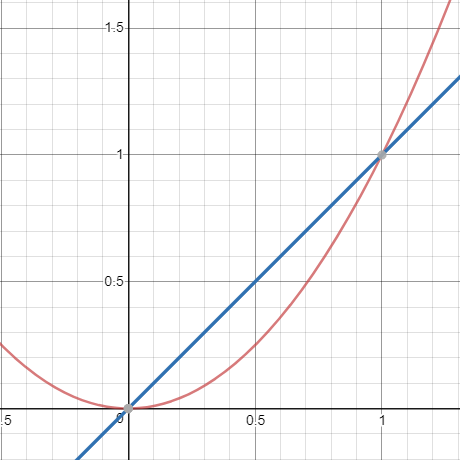
\includegraphics[width=\linewidth]{./figures/fp-1.png}
	\caption{fixed point orbits $\{0,1\}$ of $f(x)=x^{2}$}
   	\end{subfigure}
\end{figure} 

Another type of orbit is called the \textit{eventually fixed} orbit.  the orbit of some point $x_0$ is \textit{eventually fixed} if $x_0$ itself is not fixed or periodic, but some point on the orbit of $x_0$ is fixed or periodic.  For example, given the function: 
$$f^{n}(x_0)=\frac{x_0}{2^{n}}$$
Given any $x_0 \neq 0$, as $n \rightarrow \infty$, the sequence $\{ \frac{1}{2^{n}} \}$ tends towards 0.  So we can say, the orbit of $x_0$ converges to the fixed point 0, and thus is \textit{eventually fixed}. \\ 

Now, returning to our function $f(x)=x^{2}$, we can graphically analyze the orbits of a given point by tracing how the output of one iteration pipes into the input of the next iteration.  For example, let's choose a point $x_0$ such that $0 < x_0 < 1$, That is, between the two fixed points.  


\end{document}


















